%%
%% Copyright (c) 2019 Weitian LI <liweitianux@sjtu.edu.cn>
%% Creative Commons BY 4.0
%%

\documentclass{beamer}

\usetheme{metropolis}
\metroset{progressbar=foot}

\setbeamertemplate{section in toc}[sections numbered]
\setbeamertemplate{frametitle continuation}{(\insertcontinuationcount)}

% Solarized theme
% Credit: https://ethanschoonover.com/solarized/
\definecolor{SolBase02}{HTML}{073642}
\definecolor{SolBase3}{HTML}{fdf6e3}
\definecolor{SolOrange}{HTML}{cb4b16}
\definecolor{SolGreen}{HTML}{859900}
%
\setbeamercolor{normal text}{fg=SolBase02, bg=SolBase3}
\setbeamercolor{alerted text}{fg=SolOrange}
\setbeamercolor{example text}{fg=SolGreen}

\setsansfont{Fira Sans Light}[
  BoldFont={Fira Sans Medium}
]
\setmonofont{Fira Code Light}[
  BoldFont={Fira Code Medium}
]

\usepackage{bm}
\usepackage{newtxsf}
\newcommand{\R}[1]{\text{#1}}  % text math alphabets
\newcommand{\Ce}{\R{e}}  % constant e
\newcommand{\Ci}{\R{i}}  % constant i
\newcommand{\Cpi}{\piup}  % upright 'pi', provided by 'newtxsf' package
\newcommand{\B}[1]{\bm{\mathsf{#1}}}  % single-letter bold math
\newcommand{\D}[1]{\R{d}#1}
\newcommand{\diff}[2]{\frac{\D{#1}}{\D{#2}}}
\newcommand{\pdiff}[2]{\frac{\partial #1}{\partial #2}}

\usepackage{xeCJK}
\setCJKsansfont{Source Han Sans SC Light}[
  BoldFont={Source Han Sans SC Medium}
]
\xeCJKsetup{PunctStyle=kaiming}

\usepackage{hyperref}
\hypersetup{
  pdfstartview={Fit}
}

\usepackage{appendixnumberbeamer}
\usepackage{booktabs}
\usepackage{csquotes}

\usepackage{enumitem}
\setlist*{leftmargin=*}
\setlist[1]{labelindent=\parindent}
\setlist[itemize,1]{label=\ensuremath{\bullet}}
\setlist[itemize,2]{label=\ensuremath{\square}}

\usepackage{caption}
\captionsetup{%
  figurename={图},
  format=plain,
  labelformat=simple,
  labelsep=period,
  justification=centering,
  textfont={small},
  labelfont={small,bf},
}

\usepackage{xparse}
% Credit: https://tex.stackexchange.com/a/376366
\ExplSyntaxOn
\NewDocumentCommand{\cspace}{O{1em}}{%
  \tl_map_inline:nn {空} { \makebox[#1]{\phantom{##1}} }
}
\ExplSyntaxOff

\usepackage{siunitx}
% siunitx settings and new units
\sisetup{
  range-phrase=\text{--},
  range-units=single,
  product-units=repeat,
  list-separator={, },
  list-final-separator={, and },
  separate-uncertainty=true,
  detect-all,  % detecting fonts
}
%
\DeclareSIUnit\arcsec{arcsec}
\DeclareSIUnit\arcmin{arcmin}
\DeclareSIUnit\cMpc{cMpc}  % comoving Mpc
\DeclareSIUnit\cGpc{cGpc}  % comoving Gpc
\DeclareSIUnit\deg{deg}
\DeclareSIUnit\dyne{dyn}
\DeclareSIUnit\erg{erg}
\DeclareSIUnit\esu{esu}
\DeclareSIUnit\franklin{Fr}
\DeclareSIUnit\gauss{G}
\DeclareSIUnit\hubble{\ensuremath{\mathit{h}}}
\DeclareSIUnit\jansky{Jy}
\DeclareSIUnit\lightyear{ly}
\DeclareSIUnit\parsec{pc}
\DeclareSIUnit\rayleigh{Rayleigh}
\DeclareSIUnit\solarmass{\ensuremath{\mathrm{M}_{\odot}}}
\DeclareSIUnit\statcoulomb{statC}
\DeclareSIUnit\year{yr}
%
\DeclareSIUnit\kpc{\kilo\parsec}
\DeclareSIUnit\mJy{\milli\jansky}
\DeclareSIUnit\mK{\milli\kelvin}
\DeclareSIUnit\Gpc{\giga\parsec}
\DeclareSIUnit\Gyr{\giga\year}
\DeclareSIUnit\Mpc{\mega\parsec}
\DeclareSIUnit\Myr{\mega\year}
\DeclareSIUnit\uG{\micro\gauss}

\usepackage{journalabbrv}

% Fix the color of notes on the second screen
% XXX: breaks 'standout'
%\makeatletter
%\def\beamer@framenotesbegin{%
%  \usebeamercolor[fg]{normal text}%
%  \gdef\beamer@noteitems{}%
%  \gdef\beamer@notes{}%
%}
%\makeatother

\usepackage[%
  backend=biber,
  style=numeric,
  sorting=none,
  autocite=superscript,
]{biblatex}
%
% Credit: https://tex.stackexchange.com/a/60923
\DeclareCiteCommand{\cite}[\mkbibsuperscript]%
  {\iffieldundef{prenote}
     {}
     {\BibliographyWarning{Ignoring prenote argument}}%
   \iffieldundef{postnote}
     {}
     {\BibliographyWarning{Ignoring postnote argument}}}
  {\usebibmacro{citeindex}%
   \bibopenbracket\usebibmacro{cite}\bibclosebracket}
  {\supercitedelim}
  {}
\newcommand{\citeay}[1]{\citeauthor{#1} \citeyear{#1} \parencite{#1}}

\AtBeginBibliography{
  \linespread{1.1}
  \small
}
\addbibresource{../references.bib}

\graphicspath{
  {./}
  {figures/}
  {../figures/}
  {../figures/self/}
  {../sjtuthesis/}
}

% Change 'emph' style to bold face
\let\emph\relax  % there's no \RedeclareTextFontCommand
\DeclareTextFontCommand{\emph}{\boldmath\bfseries}

\newcommand{\email}[1]{\href{mailto:#1}{\texttt{#1}}}
\newcommand{\doi}[1]{\href{https://doi.org/#1}{\textsc{doi}:#1}}
\newcommand{\ads}[1]{\href{http://adsabs.harvard.edu/abs/#1}{\textsc{ads}:#1}}
\newcommand{\arxiv}[1]{\href{https://arixv.org/abs/#1}{\textsc{arXiv}:#1}}


%=====================================================================

\title[探测宇宙再电离时期]{%
  射电晕对宇宙再电离探测的影响和\texorpdfstring{\\}{}%
  基于深度学习的再电离信号分离新算法%
}
\author[李维天]{李维天 <\email{liweitianux@sjtu.edu.cn}>}
\institute{%
  物理与天文学院\\%
  上海交通大学%
}
\date{2019 年 ?? 月 ?? 日}
\subject{博士学位论文答辩}
\titlegraphic{%
  
\includegraphics[height=0.75cm]{sjtubadge}%
  \hspace{2mm}%
  
\includegraphics[height=0.75cm]{sjtulogo}%
}


%=====================================================================

\begin{document}

\maketitle

\begin{frame}{目\cspace{}录}
  \tableofcontents[hideallsubsections]
\end{frame}


%=====================================================================
\section{绪论}

%............
\begin{frame}{研究背景}
  \begin{itemize}
    \item 宇宙的中期历史仍然知之甚少,可细分为 \cite{koopmans2015}:
      无知时期 ($z \sim \numrange{200}{1100}$)、
      黑暗时期 ($z \sim \numrange{30}{200}$)、
      黎明时期 ($z \sim \numrange{15}{30}$)、
      再电离时期 (EoR; $z \sim \numrange{6}{15}$).
    \item 中性氢 21\,cm 谱线 ($\sim$\,\SI{1420}{\MHz})
      是探测 EoR 以及更早的黑暗时期的最直接而有效的探针.
  \end{itemize}

  \begin{figure}
    \centering
    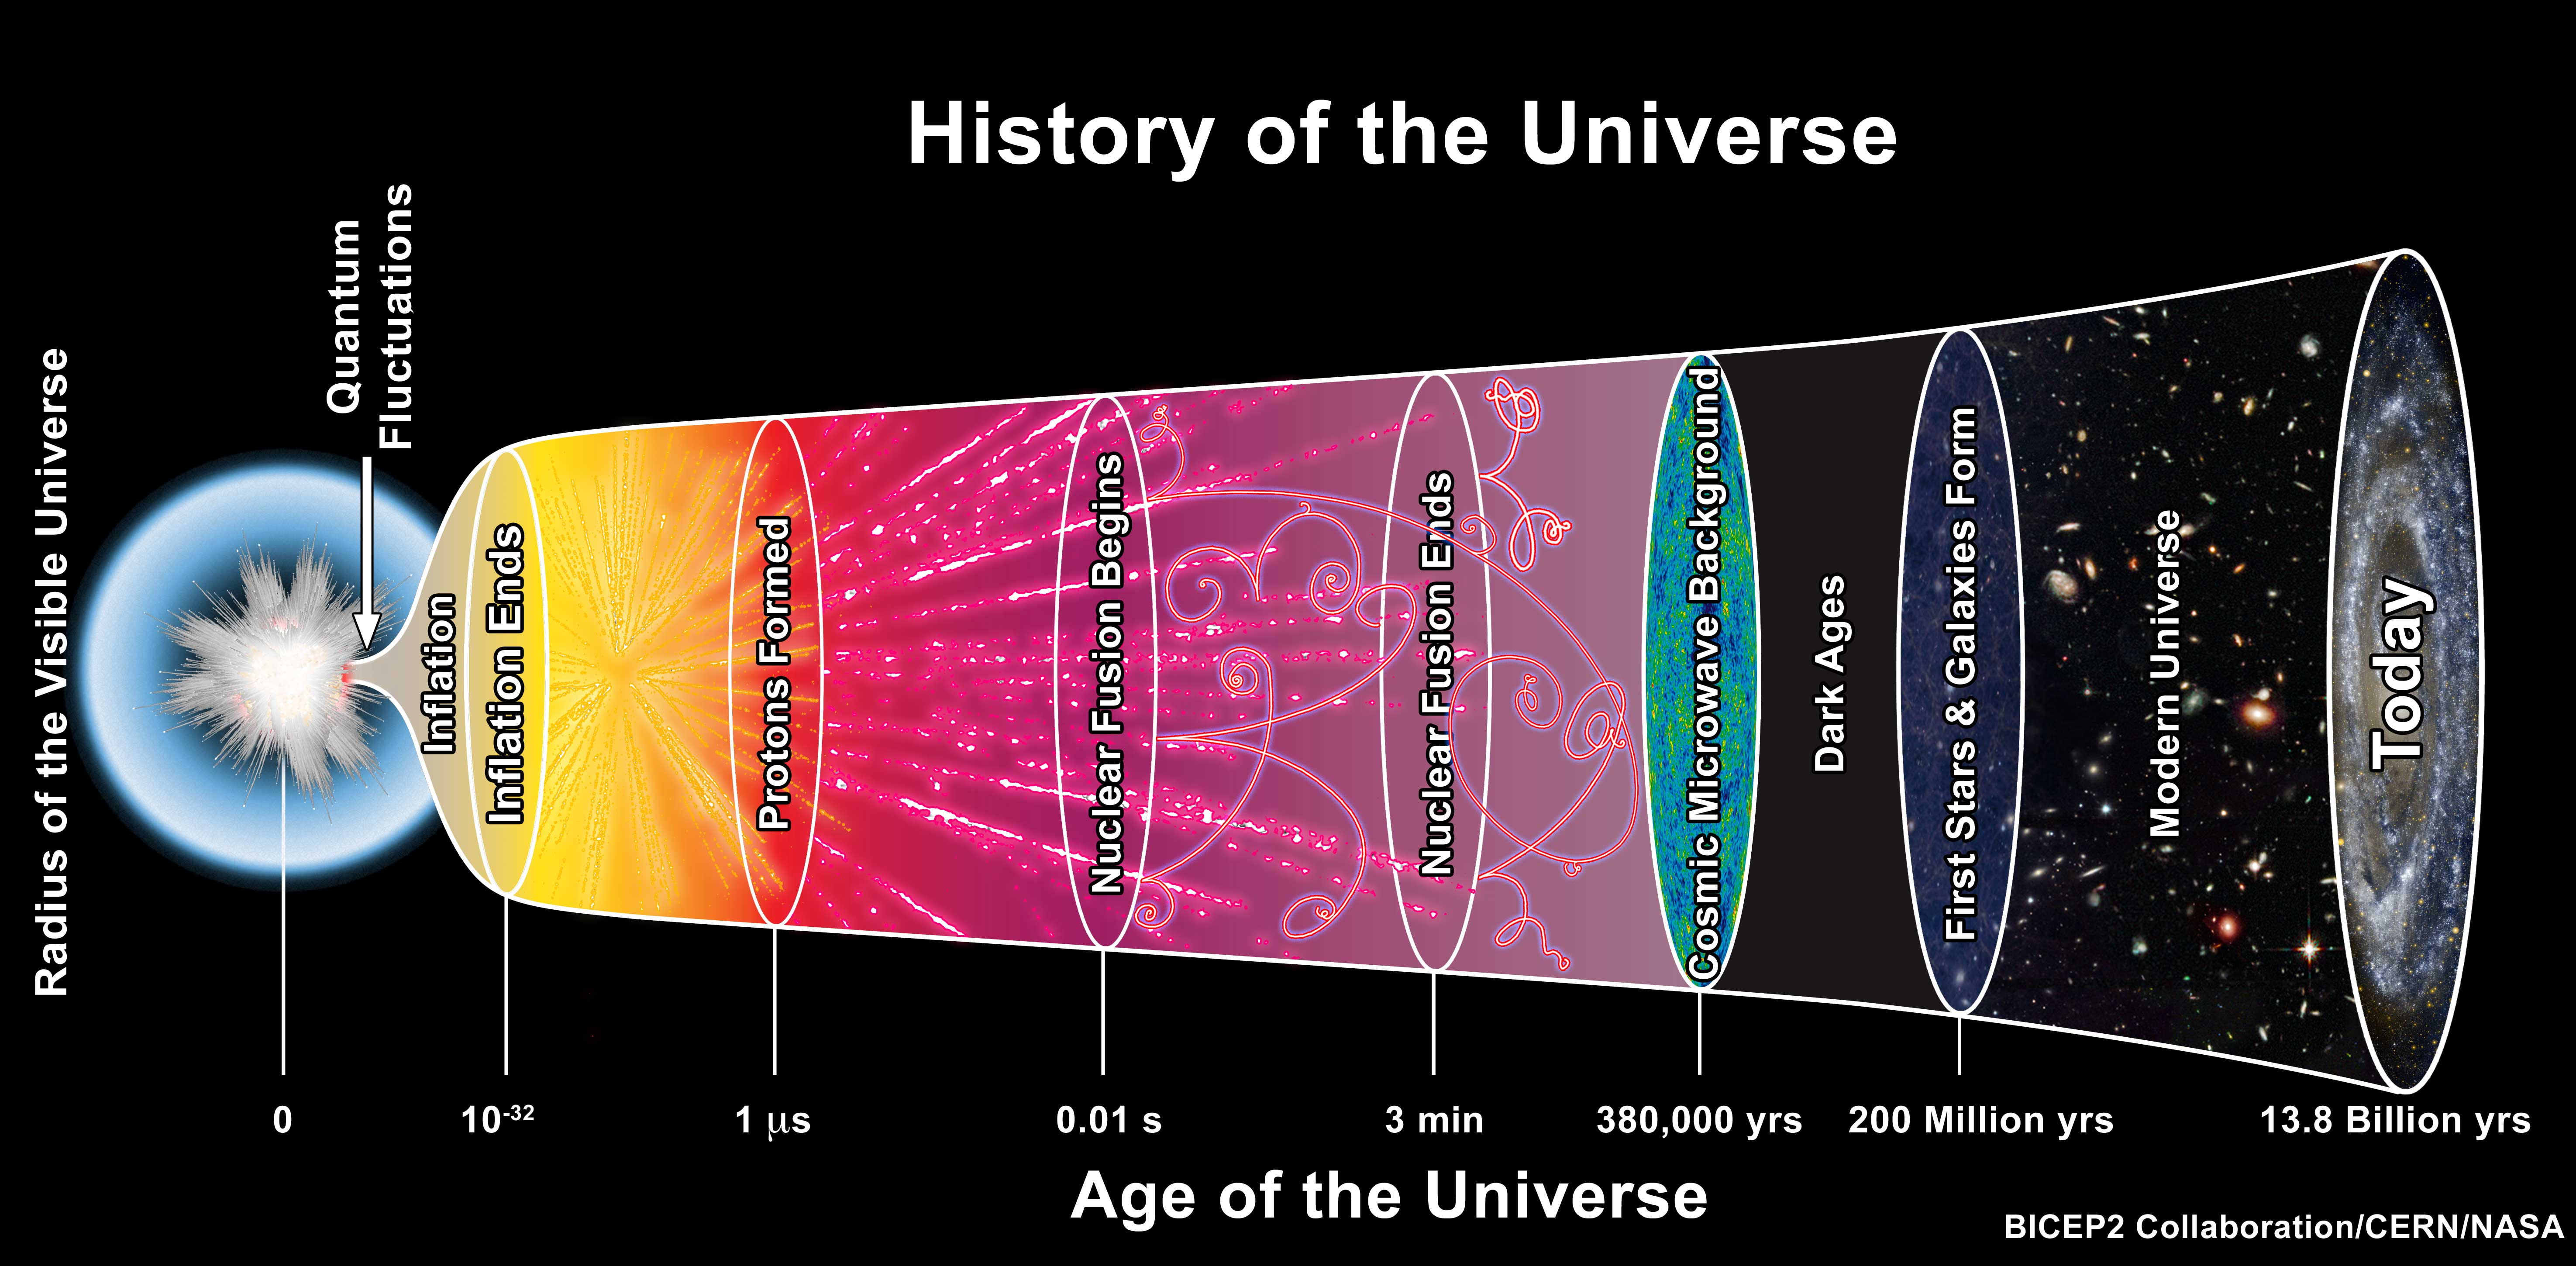
\includegraphics[width=0.8\textwidth]{universe-history}
    \caption{宇宙的演化历史. (来源: BICEP2/CERN/NASA)}
  \end{figure}
\end{frame}

%............
\begin{frame}{研究背景}
  \begin{itemize}
    \item EoR 信号应出现在 $\sim$\,\SIrange{90}{200}{\MHz} 的低频射电波段.
    \item 信号非常微弱,亮温度仅约几 mK 至十几 mK.
    \item 强烈的前景干扰(比 EoR 信号强约 5 个数量级),多种前景干扰成分.
    \item 仪器效应复杂、观测干扰显著、数据处理困难、等等.
    \item 亟待深入理解前景干扰,构建准确的前景模型,
      研发有效的前景处理和 EoR 信号提取算法,
      才能保障 EoR 探测实验的成功.
  \end{itemize}
\end{frame}

%............
\begin{frame}{研究内容}
  \begin{alertblock}{1. 改进射电晕的建模以及评估其对 EoR 探测的影响}
    \begin{itemize}
      \item 星系团射电晕是一类典型的河外射电展源:
        尺度较大(若干角分)、形态相对复杂、
        数目较多(SKA 将发现约 2500 个 \cite{cassano2015}),
        可能对 EoR 信号的探测产生显著干扰.
      \item 相比银河系以及河外点源等前景成分,对射电晕的研究明显不足而且比较粗糙.
      \item 基于\alert{湍流再加速模型},模型星系团的形成与演化过程,
        显著改进射电晕的低频射电天图的模拟.
      \item 采用 \alert{SKA1-Low 阵列布局},整合逼真的干涉阵列仪器效应.
      \item 利用一维和二维功率谱,量化射电晕对 EoR 信号的干扰情况,
        指导 EoR 实验的数据处理以及 EoR 信号分离算法的研发.
    \end{itemize}
  \end{alertblock}
\end{frame}

%............
\begin{frame}{研究内容}
  \begin{alertblock}{2. 基于深度学习研发 EoR 信号分离新算法}
    \begin{itemize}
      \item 传统的前景处理方法依赖于:前景辐射的频谱必须非常光滑.
      \item 干涉阵列的波束存在频率依赖效应,导致前景辐射的频谱出现小尺度涨落,
        光滑性受到损坏.
      \item 波束形状非常复杂,难以为现有方法打造一个实际可用的波束模型.
      \item 深度学习方法能从数据中学习知识并自适应地优化自身模型.
      \item 基于深度学习方法研发 EoR 信号分离新算法更加可行、更具有吸收力.
    \end{itemize}
  \end{alertblock}
\end{frame}


%=====================================================================
\section{射电天文学基础}

%............
\begin{frame}{射电天文学}
  \alert{射电天文学}:
  在射电波段对天体和宇宙开展研究的天文学分支.
  \alert{射电窗口}的频率范围 $\sim$ \SI{10}{\MHz} -- \SI{1000}{\GHz}
  (波长 $\sim$ \SI{0.3}{\mm} -- \SI{30}{\meter}).

  \begin{figure}
    \centering
    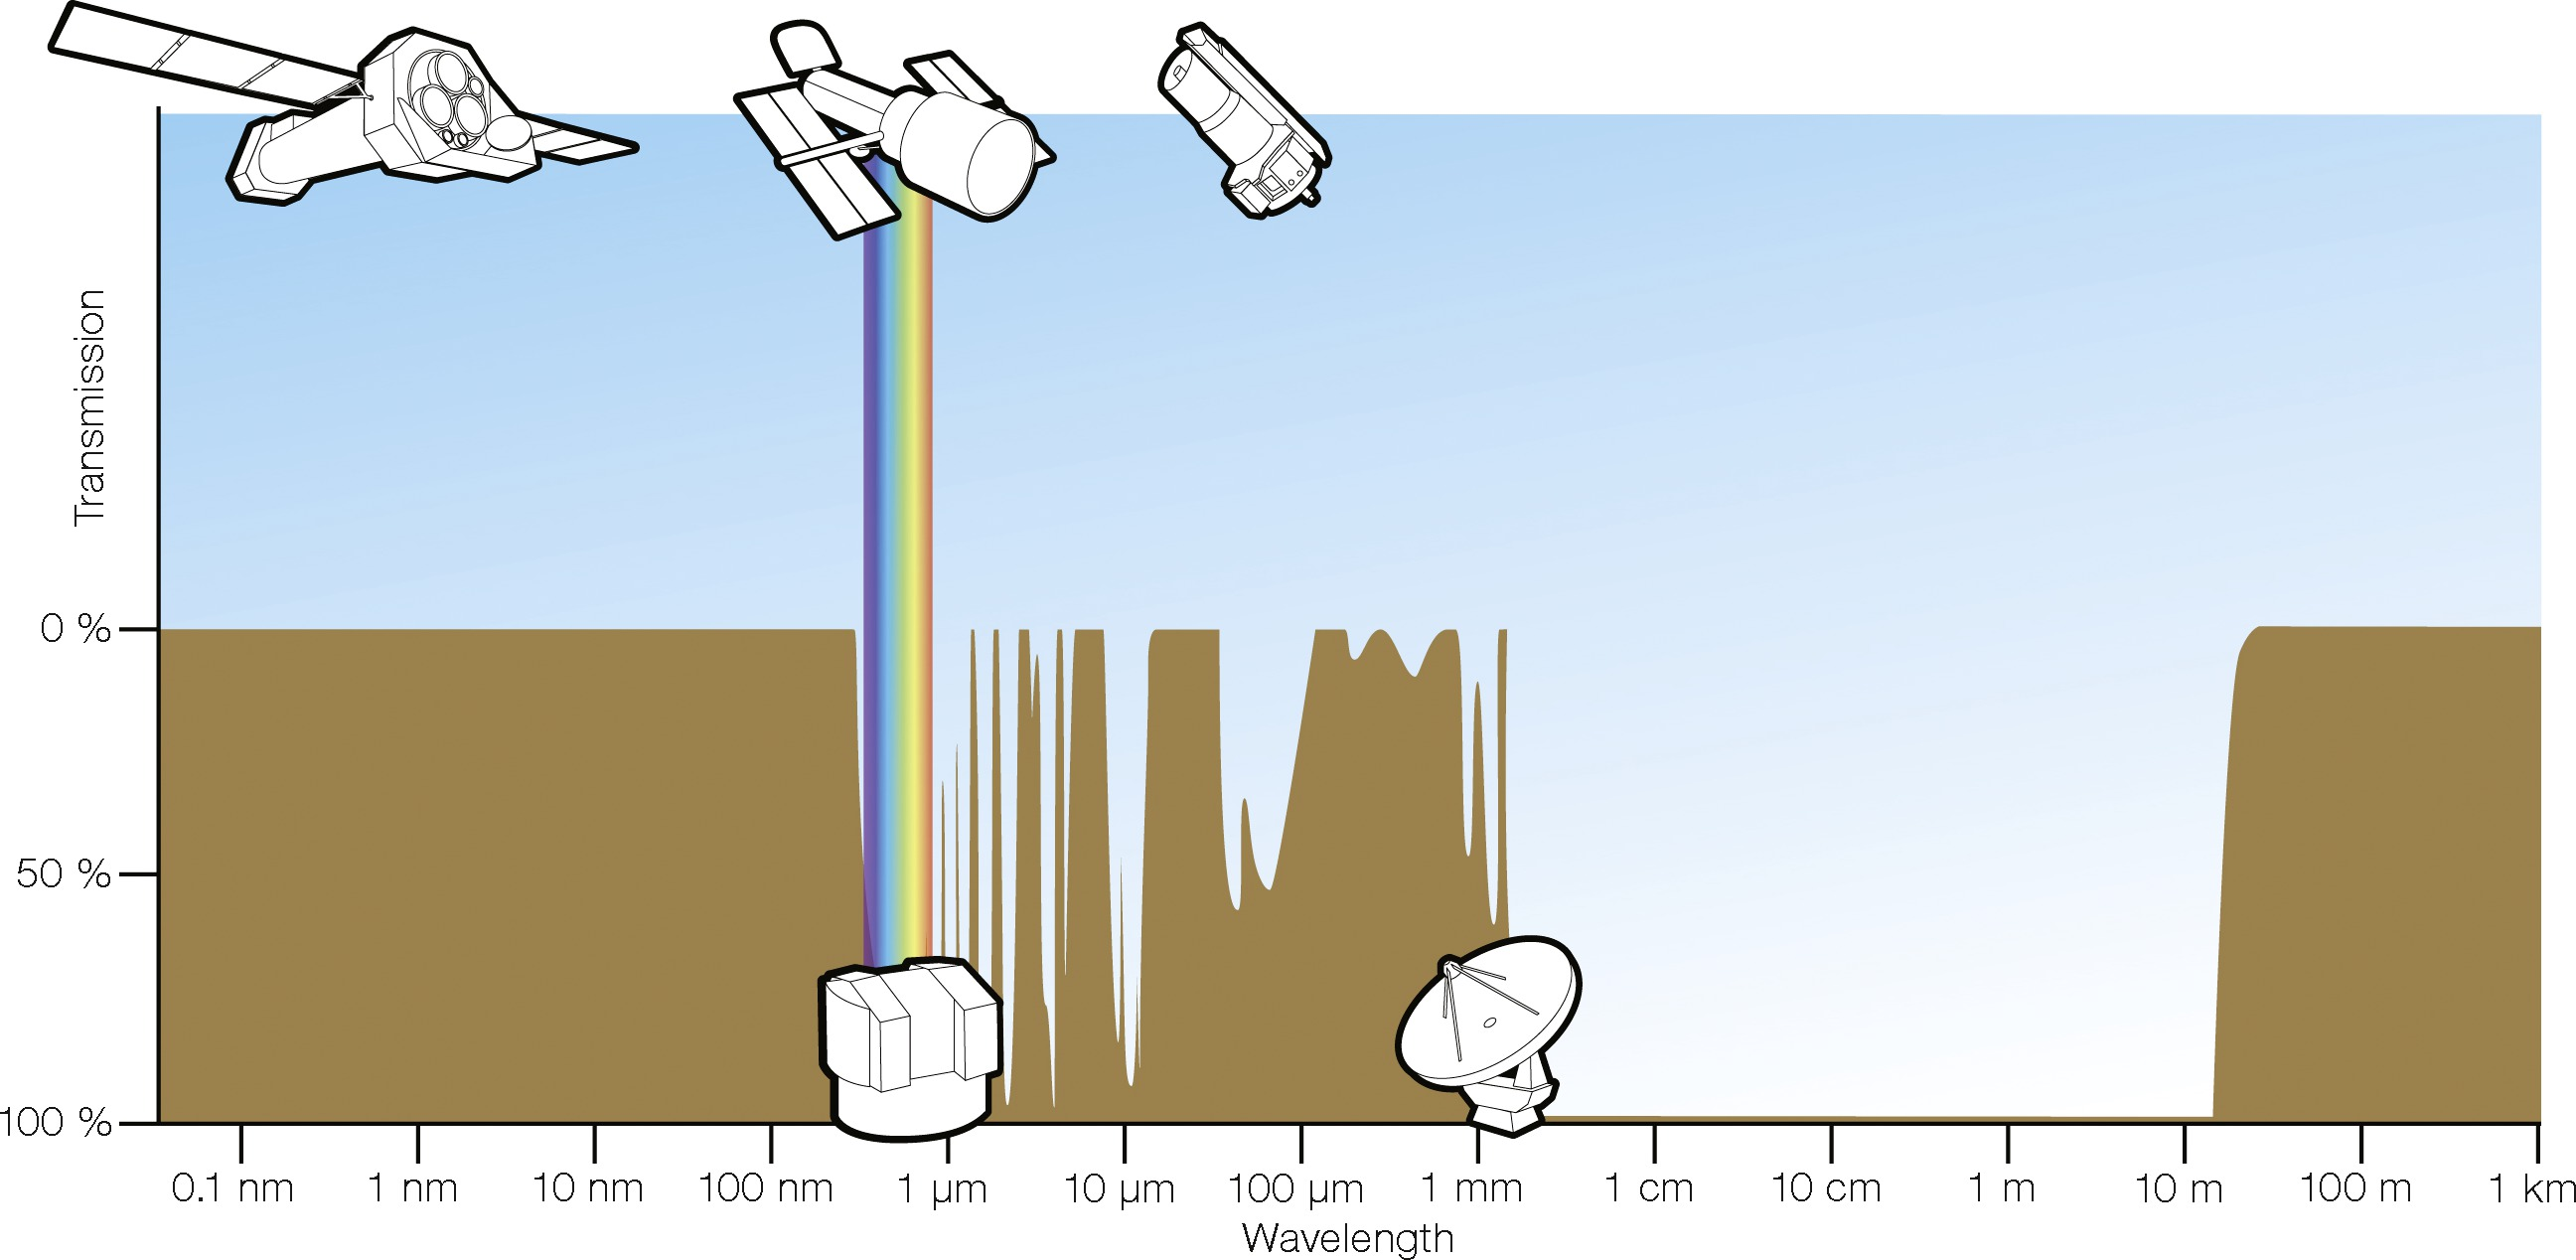
\includegraphics[width=\textwidth]{atmospheric-em-transmittance}
    \caption{大气层的电磁辐射透射率. (来源: \citeay{condon2016})}
  \end{figure}
\end{frame}

%............
\begin{frame}{比强度和流量密度}
  \begin{columns}
    \column{0.6\textwidth}
      \begin{alertblock}{比强度 (specific intensity)}
        \smallskip
        单位频率间隔内、沿着辐射传播方向上单位立体角穿过垂直于传播方向的单位面积
        的辐射功率,即:
        \begin{equation}
          I_{\nu} \equiv
            \frac{\D{P_{\nu}}}{(\cos\theta\,\D{\sigma})
              \,\D{\nu} \,\D{\Omega}} \,,
        \end{equation}
        亦被称为\emph{谱亮度},或简称\emph{强度}或\emph{亮度}.
      \end{alertblock}

      \begin{alertblock}{流量密度 (flux density)}
        \smallskip
        \begin{equation}
          S_{\nu} \equiv
            \int_{\R{source}} I_{\nu}(\theta,\phi) \cos\theta \,\D{\Omega} ,
        \end{equation}
        单位为 \si{\jansky},
        $\SI{1}{\jansky} = \SI{e-26}{\watt\per\square\meter\per\hertz}$.
      \end{alertblock}

    \column{0.4\textwidth}
      \begin{figure}
        \centering
        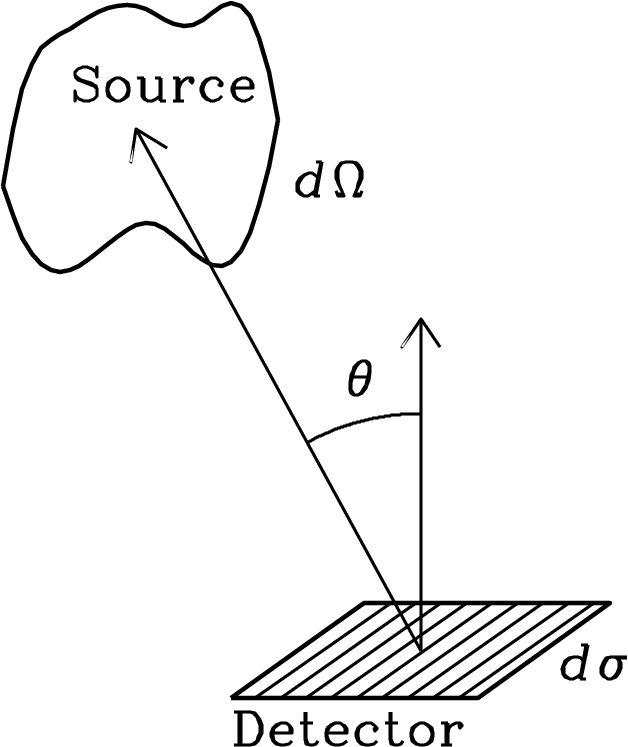
\includegraphics[width=0.9\columnwidth]{specific-intensity}
        \caption{比强度 $I_{\nu}$ 测量示意图. (\citeay{condon2016})}
      \end{figure}
  \end{columns}
\end{frame}

%............
\begin{frame}{辐射转移}
  \begin{itemize}
    \item 辐射在介质中传播时会经历吸收和发射,由\alert{辐射转移方程}描述:
      \begin{equation}
        \diff{I_{\nu}}{s} = -\kappa I_{\nu} + j_{\nu} ,
      \end{equation}
      其中 $\kappa$ 为吸收系数, $j_{\nu}$ 为发射系数.
    \item \alert{光深}:
      \begin{equation}
        \tau \equiv
          - \int_{s_{\R{out}}}^{s_{\R{in}}} \kappa(s') \,\D{s'} .
      \end{equation}
      当 $\tau \ll 1$ 时,称介质是\emph{光学薄}的;
      当 $\tau \gg 1$ 时,则称介质是\emph{光学厚}的.
  \end{itemize}
\end{frame}

%............
\begin{frame}{亮温度 $T_b$}
  \begin{itemize}
    \item \alert{黑体辐射}的频谱 $B_{\nu}(\nu, T)$ 只取决于其温度 $T$,
      由 \alert{Planck 定律}给出:
      \begin{equation}
        B_{\nu}(\nu, T) =
          \frac{2 h_p \nu^3}{c^2} \left[ \exp\left(
            \frac{h_p \nu}{k_B T} \right) - 1 \right]^{-1} .
      \end{equation}
    \item 在射电波段有 $h_p \nu \ll k_B T$,于是有 \alert{Rayleigh--Jeans 近似}:
      \begin{equation}
        B_{\nu}(\nu, T) \approx \frac{2 \nu^2 k_B T}{c^2} .
      \end{equation}
      黑体的亮度 $B_{\nu}$ 与其温度 $T$ 严格成正比.
    \item 一个辐射源的亮度 $I_{\nu}$ 可以很方便与使用\alert{亮温度}来描述:
      \begin{equation}
        T_b(\nu) \equiv \frac{I_{\nu} c^2}{2 k_B \nu^2} .
      \end{equation}
  \end{itemize}
\end{frame}

%............
\begin{frame}{干涉测量原理}
  \begin{columns}
    \column{0.4\textwidth}
    二元准单色干涉仪观测一个点源,相关器的输出响应为:
    \begin{align}
      R & = \langle V_1(t) V_2(t) \rangle \\
        & = \frac{1}{2} V^2 \cos (\omega \tau_g) ,
    \end{align}
    $\tau_g = \B{b} \cdot \hat{\B{s}}$ 为几何延迟,\\
    $\B{b}$ 为基线矢量,\\
    $\hat{\B{s}}$ 为辐射源的方向.

    \column{0.6\textwidth}
    \begin{figure}
      \centering
      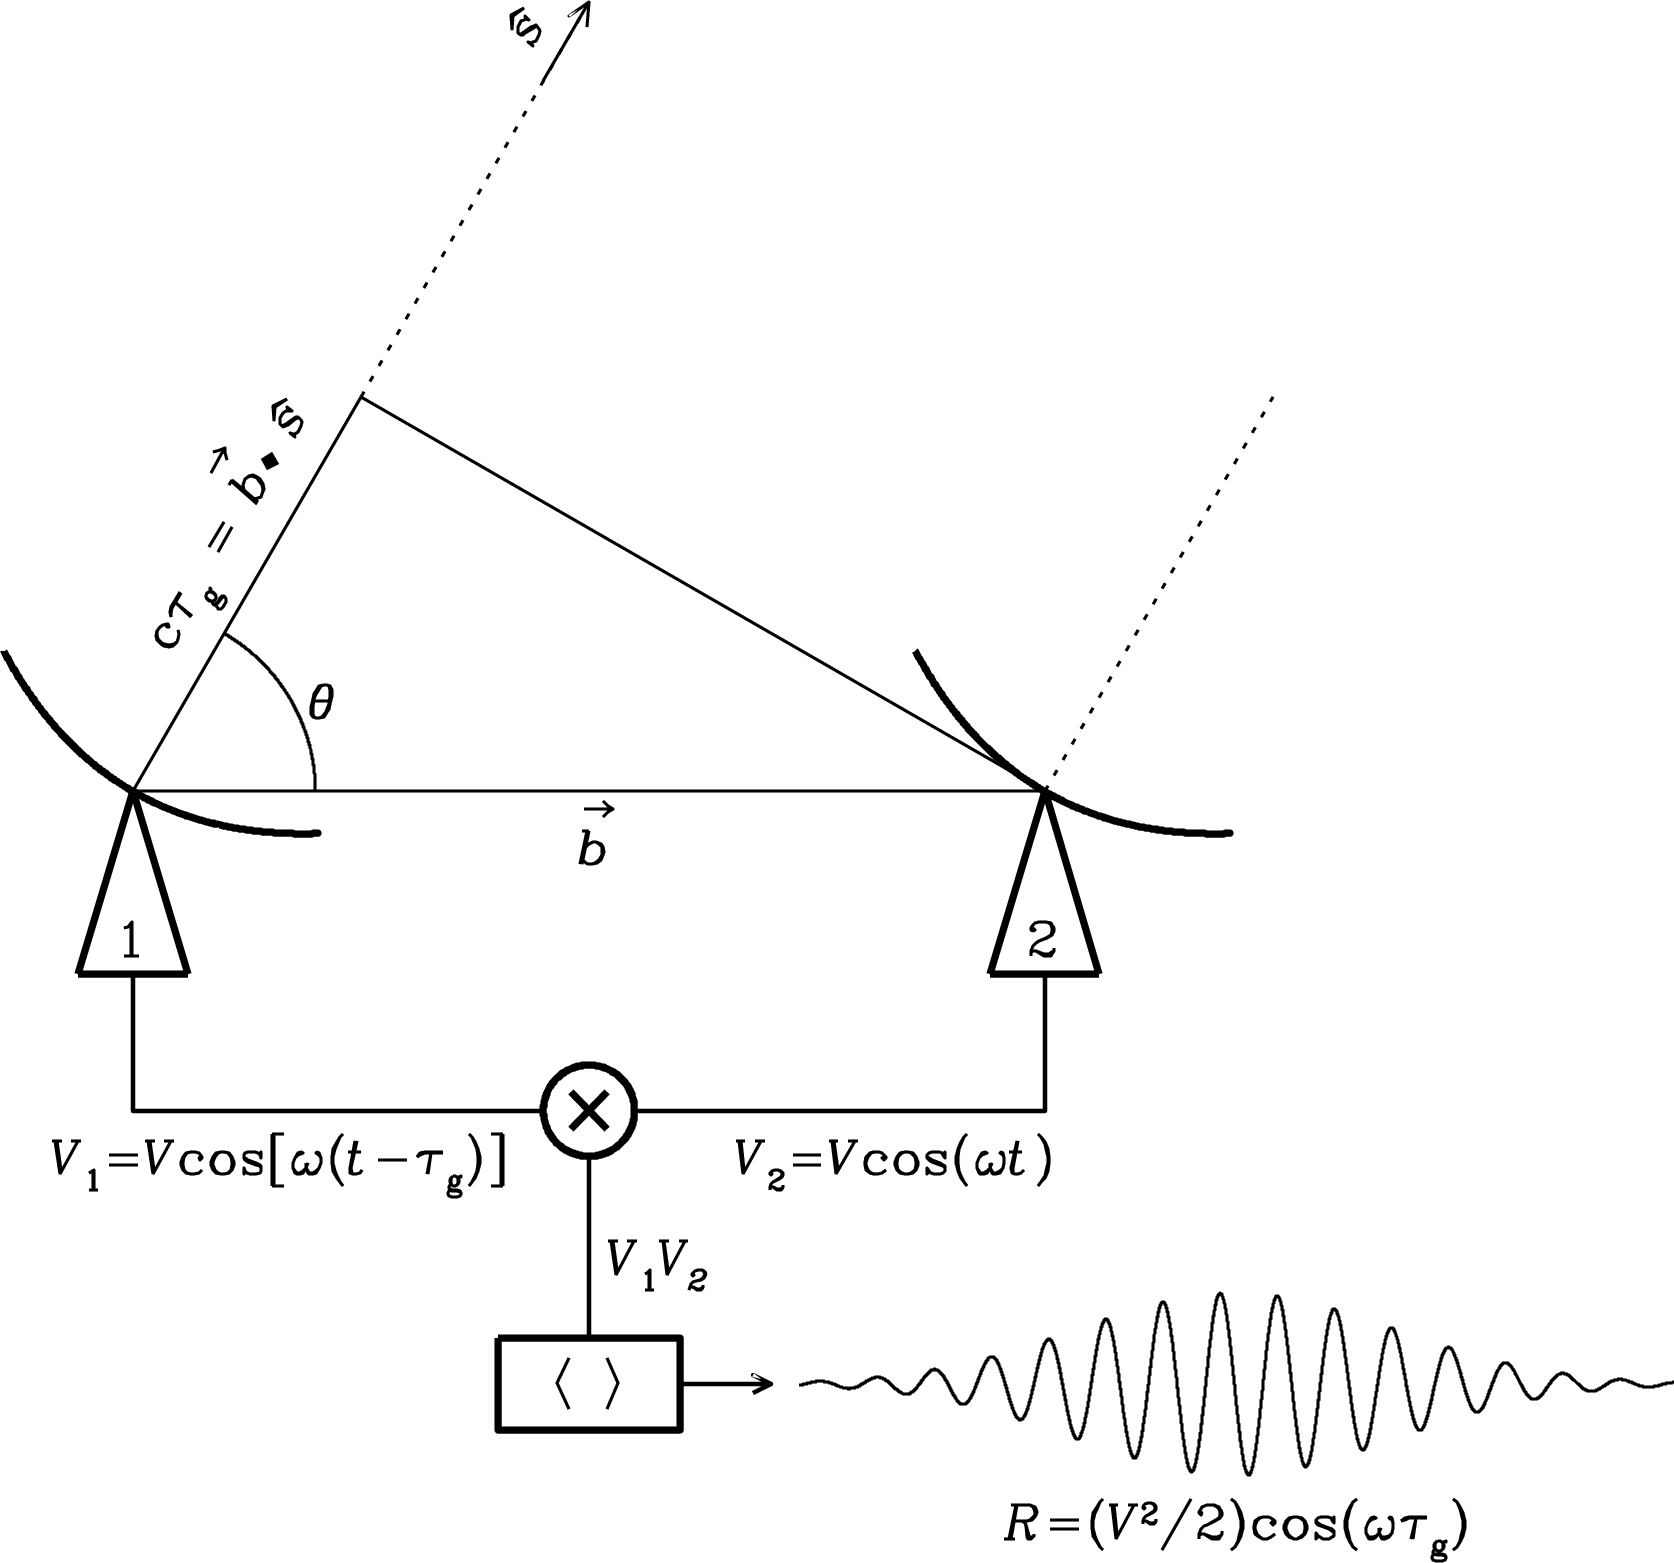
\includegraphics[width=\columnwidth]{interferometer}
      \caption{二元准单色干涉仪示意图. (\citeay{condon2016})}
    \end{figure}
  \end{columns}
\end{frame}

%............
\begin{frame}{干涉测量原理}
  \begin{itemize}
    \item 一个展源 $I_{\nu}(\hat{\B{s}})$ 可当作一系列独立的点源处理,
      于是干涉仪响应为:
      \begin{equation}
        R_c = \int I_{\nu}(\hat{\B{s}})
          \cos (2\Cpi\, \B{b} \cdot \hat{\B{s}} / \lambda) \,\D{\Omega} .
      \end{equation}
    \item 上述 \enquote{cosine} 相关器只能测量 $I_{\nu}(\hat{\B{s}})$ 的偶成分.
    \item 为测量 $I_{\nu}(\hat{\B{s}})$ 的奇成分,
      还需要一个 \enquote{sine} 相关器,
      可通过对其中一个天线的输出增加 $\Cpi/2$ 的相位延迟来实现,于是:
      \begin{equation}
        R_s = \int I_{\nu}(\hat{\B{s}})
          \sin (2\Cpi\, \B{b} \cdot \hat{\B{s}} / \lambda) \,\D{\Omega} .
      \end{equation}
    \item \alert{复可见度 (complex visibility)} 定义为:
      \begin{equation}
        \mathcal{V}
          \equiv R_c - \Ci R_s
          = \int I_{\nu}(\hat{\B{s}})
            \exp (- 2\Cpi\Ci\, \B{b} \cdot \hat{\B{s}} / \lambda)
            \,\D{\Omega} .
      \end{equation}
  \end{itemize}
\end{frame}

%............
\begin{frame}{坐标系统}
  \begin{columns}
    \column{0.55\textwidth}
    \begin{itemize}
      \item $w$ 轴指向参考方向,通常为目标的中心; \\
        $u$ 轴向东; \\
        $v$ 轴向北.
      \item 基线矢量: $\B{b} = (u,v,w) \,\lambda$.
      \item 方向矢量: $\hat{\B{s}} = \left( l, m, \sqrt{1-l^2-m^2} \right)$,
        其中 $l, m$ 分别为 $\hat{\B{s}}$ 对 $u, v$ 轴的投影长度.
    \end{itemize}

    \column{0.4\textwidth}
    \begin{figure}
      \centering
      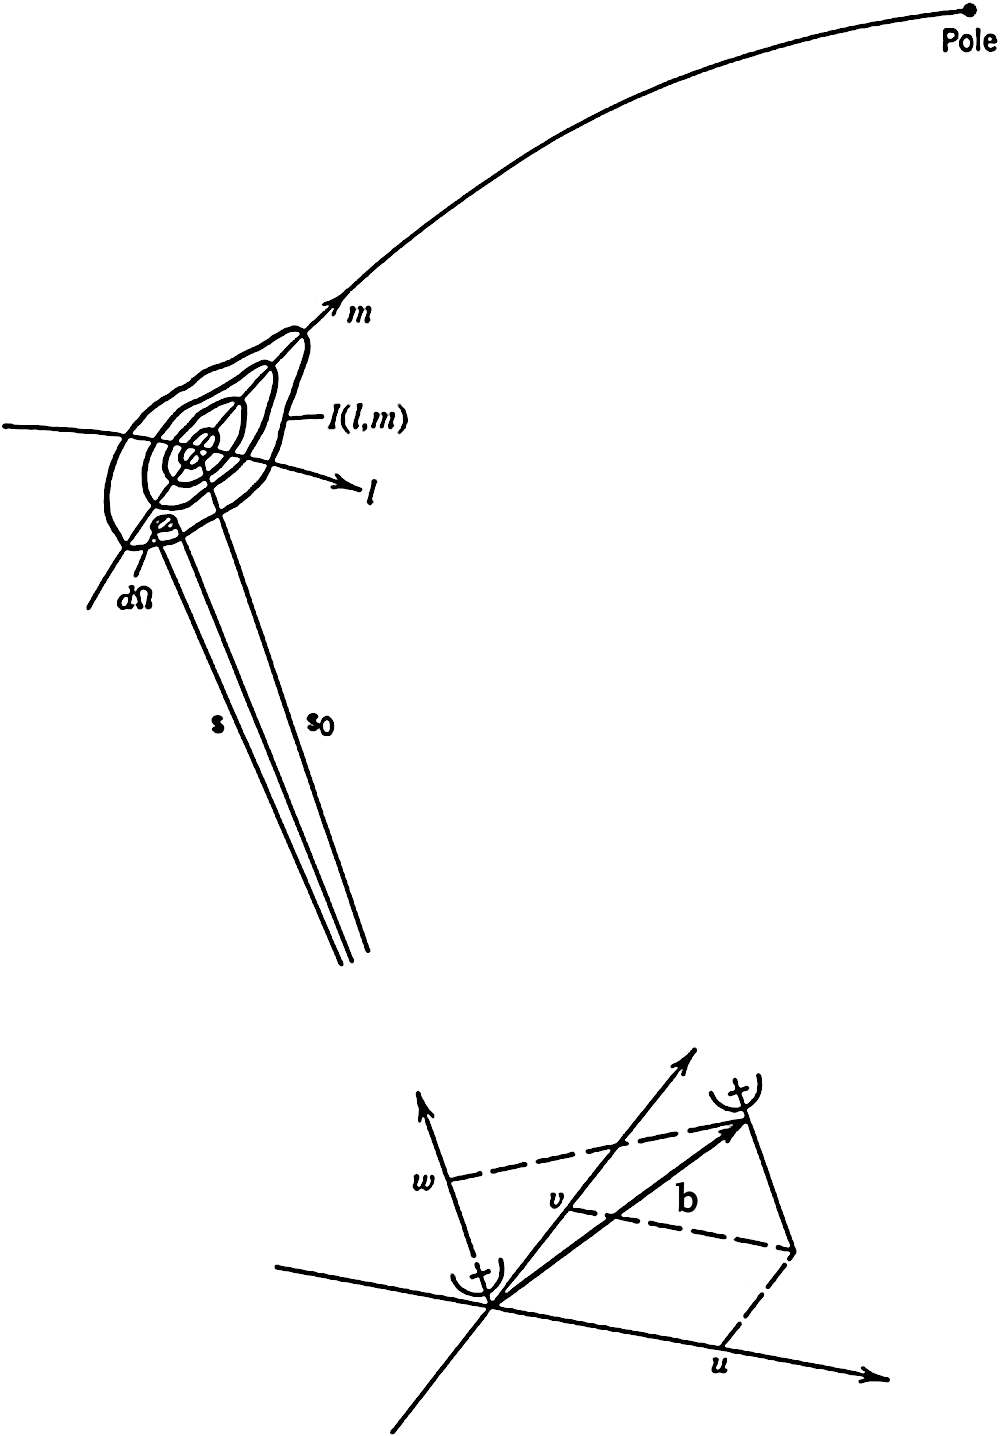
\includegraphics[width=\columnwidth]{interferometer-coordsys}
      \caption{干涉仪的 $(u,v,w)$ 直角坐标系. (\citeay{thompson2017})}
    \end{figure}
  \end{columns}
\end{frame}

%............
\begin{frame}{成像原理}
  \begin{equation}
    \mathcal{V}(u,v,w)
      = \!\iint \!\frac{I_{\nu}(l,m)}{\sqrt{1-l^2-m^2}}
      \exp \!\left[ -2\Cpi\Ci \!\left( ul+vm+w\sqrt{1-l^2-m^2} \right) \right]
      \D{l}\,\D{m}
  \end{equation}

  \begin{itemize}
    \item 注意,上式\alert{不是}二维 Fourier 变换.
    \item 在以下两种常见的特殊情况下:
      \begin{itemize}
        \item 所有基线矢量共面,即有 $w = 0$;
        \item 小视场成像,即满足 $\big| \Cpi w(l^2+m^2) \big| \ll 1$.
      \end{itemize}
      上式可近似成二维 Fourier 变换:
      \begin{equation}
        \mathcal{V}(u,v)
          = \iint \frac{I_{\nu}(l,m)}{\sqrt{1-l^2-m^2}}
            \exp [-2\Cpi\Ci\, (ul+vm)] \,\D{l}\,\D{m},
      \end{equation}
    \item 通过逆变换,可得目标的亮度分布 $I_{\nu}(l,m)$:
      \begin{equation}
        \frac{I_{\nu}(l,m)}{\sqrt{1-l^2-m^2}}
          = \iint \mathcal{V}(u,v)
            \exp [2\Cpi\Ci\, (ul+vm)] \,\D{l}\,\D{m}.
      \end{equation}
  \end{itemize}
\end{frame}

%............
\begin{frame}{$uv$ 覆盖}
  \begin{itemize}
    \item 基线 $\B{b} = (u,v,w) \,\lambda$ 每个时刻测量一对可见度数据: \\
      $\mathcal{V}(u,v)$ 和 $\mathcal{V}(-u,-v)$.
    \item \alert{$uv$ 覆盖}指 $uv$ 平面内被测量到的范围,
      由\alert{采样函数} $S(u,v)$ 描述.
    \item 对测量的可见度数据进行逆 Fourier 变换,
      仅能得到目标的\alert{脏图 (dirty map)}:
      \begin{equation}
        \frac{I_{\nu}^D(l,m)}{\sqrt{1-l^2-m^2}}
          = \iint \mathcal{V}(u,v) S(u,v)
            \exp [2\Cpi\Ci\, (ul+vm)] \,\D{l}\,\D{m}.
      \end{equation}
    \item \alert{综合波束 (synthesized beam)}
      或\alert{点扩散函数 (point spread function; PSF)}
      是 $S(u,v)$ 的 Fourier 变换:
      \begin{equation}
        B(l,m) = \iint S(u,v) \exp [2\Cpi\Ci\, (ul+vm)] \,\D{l}\,\D{m}.
      \end{equation}
  \end{itemize}
\end{frame}

%............
\begin{frame}{成像过程的变换关系}
  \begin{figure}
    \centering
    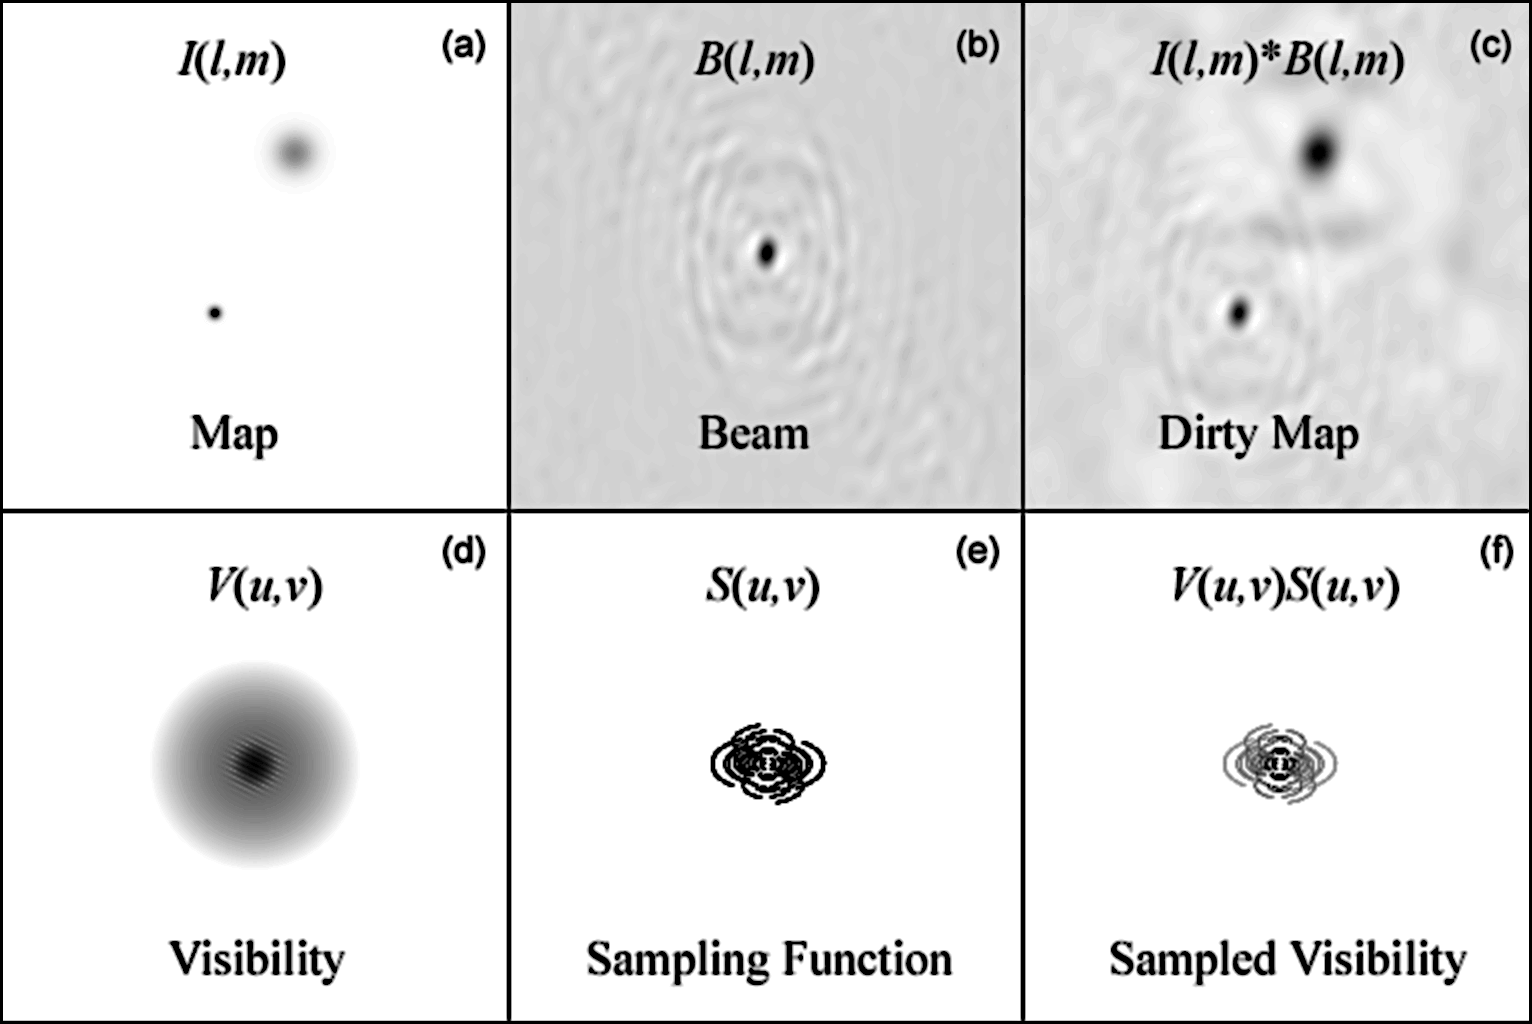
\includegraphics[width=0.9\textwidth]{imaging-relations}
    \caption{%
      (a) 真实图像;
      (b) 综合波束;
      (c) 脏图;
      (d) 真实的可见度数据;
      (e) 采样函数;
      (f) 测量到的可见度数据.
      (Dale E. Gary, Radio Astronomy)
    }
  \end{figure}
\end{frame}


%=====================================================================
\section{总结}

\begin{frame}{结\cspace{}论}
  结论...
\end{frame}

\begin{frame}{已发表论文}
  \small
  \begin{itemize}
    \item
      \textsc{\alert{Li, Weitian}; Xu, Haiguang; Ma, Zhixian; Hu, Dan;
      Zhu, Zhenghao; Shan, Chenxi; Wang, Jingying; Gu, Junhua;
      Zheng, Dongchao; Lian, Xiaoli; Zheng, Qian; Wang, Yu;
      Zhu, Jie; Wu, Xiang-Ping}.
      \enquote{\it Contribution of Radio Halos to the Foreground for
        SKA EoR Experiments,}
      \href{http://adsabs.harvard.edu/abs/arXiv:1905.05399}{%
        2019, ApJ, accepted}
    \item
      \textsc{\alert{Li, Weitian}; Xu, Haiguang; Ma, Zhixian; Zhu, Ruimin;
      Hu, Dan; Zhu, Zhenghao; Gu, Junhua; Shan, Chenxi; Zhu, Jie;
      Wu, Xiang-Ping}.
      \enquote{\it Separating the EoR Signal with a Convolutional Denoising
        Autoencoder: A Deep-learning-based Method,}
      \href{http://adsabs.harvard.edu/abs/2019MNRAS.485.2628L}{%
        2019, MNRAS, 485, 2628}
    \item
      合作论文 12 篇
  \end{itemize}
\end{frame}

\begin{frame}[standout]
  \Huge 谢\cspace{}谢

  \note[item]{感谢导师}
  \note[item]{感谢评审专家}
\end{frame}


%=====================================================================
\appendix

\begin{frame}[standout]
  Appendix
\end{frame}

\begin{frame}[allowframebreaks]{参考文献}
  \printbibliography[heading=none]
\end{frame}

\end{document}
